%%%%%%%%%%%%%%%%%%%%%%%%%%%%%%%%%%%%%%%%%%%%%%%%%%%%%%%%%%%%%%%%%%%%%
% LaTeX Template: Project Titlepage Modified (v 0.1) by rcx
%
% Original Source: http://www.howtotex.com
% Date: February 2014
% 
% This is a title page template which be used for articles & reports.
% 
% This is the modified version of the original Latex template from
% aforementioned website.
% 
%%%%%%%%%%%%%%%%%%%%%%%%%%%%%%%%%%%%%%%%%%%%%%%%%%%%%%%%%%%%%%%%%%%%%%

\documentclass[11pt]{report}
\usepackage[a4paper]{geometry}
\usepackage[myheadings]{fullpage}
\usepackage{fancyhdr}
\usepackage{lastpage}
\usepackage{graphicx, wrapfig, subcaption, setspace, booktabs}
\usepackage[T1]{fontenc}
\usepackage[font=small, labelfont=bf]{caption}
\usepackage{fourier}
\usepackage[protrusion=true, expansion=true]{microtype}
\usepackage[english]{babel}
\usepackage{sectsty}
\usepackage{url, lipsum}
\usepackage{amsmath}

\newcommand{\HRule}[1]{\rule{\linewidth}{#1}}
\onehalfspacing
\setcounter{tocdepth}{5}
\setcounter{secnumdepth}{5}

%-------------------------------------------------------------------------------
% HEADER & FOOTER
%-------------------------------------------------------------------------------
\pagestyle{fancy}
\fancyhf{}
\setlength\headheight{15pt}
\fancyhead[L]{Terrence Ho}
\fancyhead[R]{Experiment 3}
\fancyfoot[R]{Page \thepage\ of \pageref{LastPage}}
%-------------------------------------------------------------------------------
% TITLE PAGE
%-------------------------------------------------------------------------------

\begin{document}

\title{ \normalsize \textsc{Physics 4AL}
        \\ [2.0cm]
        \HRule{0.5pt} \\
        \LARGE \textbf{\uppercase{Experiment 3: Conservation of Mechanical Energy}}
        \HRule{2pt} \\ [0.5cm]
        \vspace*{2\baselineskip}}

\date{}

\author{
        Terrence Ho | ID: 804793446 \\ 
        Date of Lab: May 2nd, 2017 \\
        Lab Section: Tuesday, 5 P.M.\\
        T.A.: David Bauer\\
        Lab Partners: Robathan Harries}

\maketitle
\tableofcontents
\newpage

%-------------------------------------------------------------------------------
% Section title formatting
\sectionfont{\scshape}
%-------------------------------------------------------------------------------

%-------------------------------------------------------------------------------
% BODY
%-------------------------------------------------------------------------------

\section*{Discussion}
\addcontentsline{toc}{section}{Discussion}

We aligned the photocomb at the 36th tooth from the left.  We then
correspondingly always pulled the glider to the left when performing our
experiment.  

Potential energy of a spring is given by the equation \(F = -kx\), where \(F\) is the force
exerted on the spring, \(k\) is the spring constant, and \(x\) is the distance pulled. 
To obtain our potential energy calculations, we first obtained the spring constant 
\(k\) by hanging a mass from the spring and measuring the distance stretched,
shown in \textbf{Figure 3.1}.  \(k\) is found to be 6.016 $\pm$ 0.001 \(N/m\).

To calculate both the kinetic and potential energy in space, block event times
were measured using the DAQ.  Because we know that each tooth and gap between
each tooth is 2 mm $\pm$ 30 $\mu$m, each block event time represented an
increase in 4 mm.  The potential energy is calculated with the average distance
$\bar{x}$ using the formula \(E_p(\bar{x}(i)) = \frac{1}{2}k\bar{x}^2\) and 
calculated \(k\).  

Velocity of the glider was calculated by differentiating displacement with respect to
time using the equation \(v(\bar{x}(i)) = \frac{x_{i+1} - x_i}{t_{i+1} - t_i}\).
Because kinetic energy \(E_k\) can be found by the formula \(E_k(\bar{x}(i)) =
\frac{1}{2}mv(\bar{x}(i))^2\), when can substitute \(v(\bar{x}(i))\) and obtain
kinetic energy with this final equation \(E_k(\bar{x}(i)) =
\frac{1}{2}m\Bigg(\frac{x_{i+1} - x_i}{t_{i+1} - t_i}\Bigg)^2\). 

We then plotted \(E_k(\bar{x}(i))\), \(E_p(\bar{x}(i))\), and
\(E_{total}(\bar{x}(i))\) on a
plot with respect to average distance $\bar{x}$.  The potential energy is an
upward facing parabola, while kinetic energy is a downward facing parabola.
When the spring is pulled, potential energy is at it's maximum and kinetic
energy is zero.  When the spring and glider system is released, potential energy
is transformed into kinetic energy and the glider gains speed, until it reaches
the equilibrium point where kinetic energy is maximized.  After, kinetic energy
is transformed once again into potential energy as the spring pulls on the
glider.  Other than a slight loss of energy to friction (shown in \textbf{Figure
3.2}), the energy level of the system remained the same.  Energy was only being
transferred between potential and kinetic energy as the glider moved.

\section*{Plots and Tables}
\addcontentsline{toc}{section}{Plots and Tables}
Mass of Glider with Photogate Comb = 0.225 $\pm$ 0.0005 kg

\begin{center}
    \begin{tabular}{| c | c | c |}
        \hline
        Hanging Mass (kg) & Applied Force (N) & Glider Displacement (m) \\
        \hline
        0.100 $\pm$ 0.0005  & 0.98 $\pm$ 0.005 & 0.162 $\pm$ 0.00005 \\
        \hline
        0.060 $\pm$ 0.0005 & 0.588 $\pm$ 0.005 & 0.099 $\pm$ 0.00005 \\
        \hline
        0.035 $\pm$ 0.0005 & 0.343 $\pm$ 0.005 & 0.056 $\pm$ 0.00005 \\
        \hline
        0.020 $\pm$ 0.0005 & 0.196 $\pm$ 0.005 & 0.032 $\pm$ 0.00005 \\
        \hline
        0.005 $\pm$ 0.0005 & 0.049 $\pm$ 0.005 & 0.008 $\pm$ 0.00005 \\
        \hline
    \end{tabular}
\end{center}
\captionof*{table}{\textbf{Table 3.1 Force exerted on spring vs displacement.}
9.8 m/s$^2$ was as the acceleration due to gravity to calculate applied force.}

\begin{figure}[h!]
    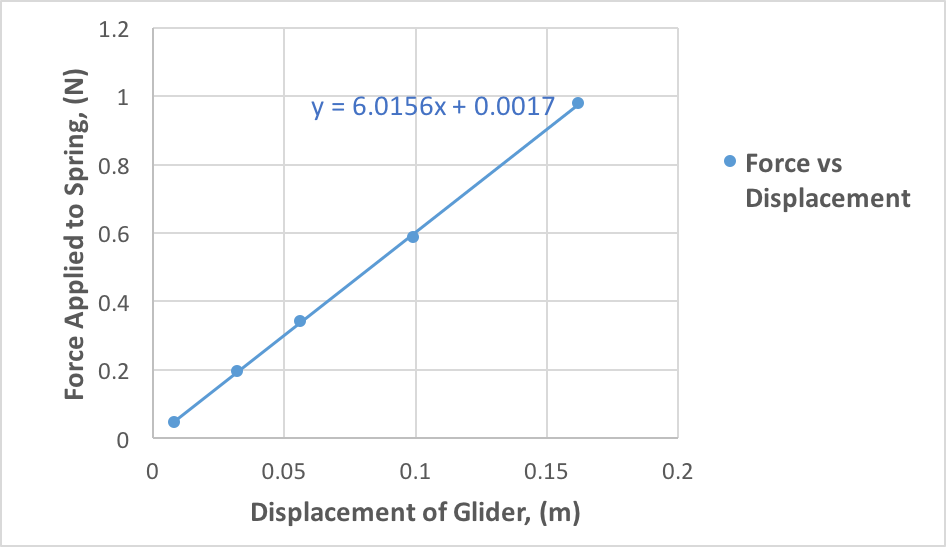
\includegraphics[width=\linewidth]{SpringForce.png}
    \captionsetup{labelformat=empty}
    \caption{\textbf{Figure 3.1 Measuring Spring Constant by comparing force
    applied by hanging mass and displacement.} The spring constant found in this
case is \(k = (6.016 \pm 0.002)\) in N/m.}
\end{figure}

\begin{figure}[h!]
    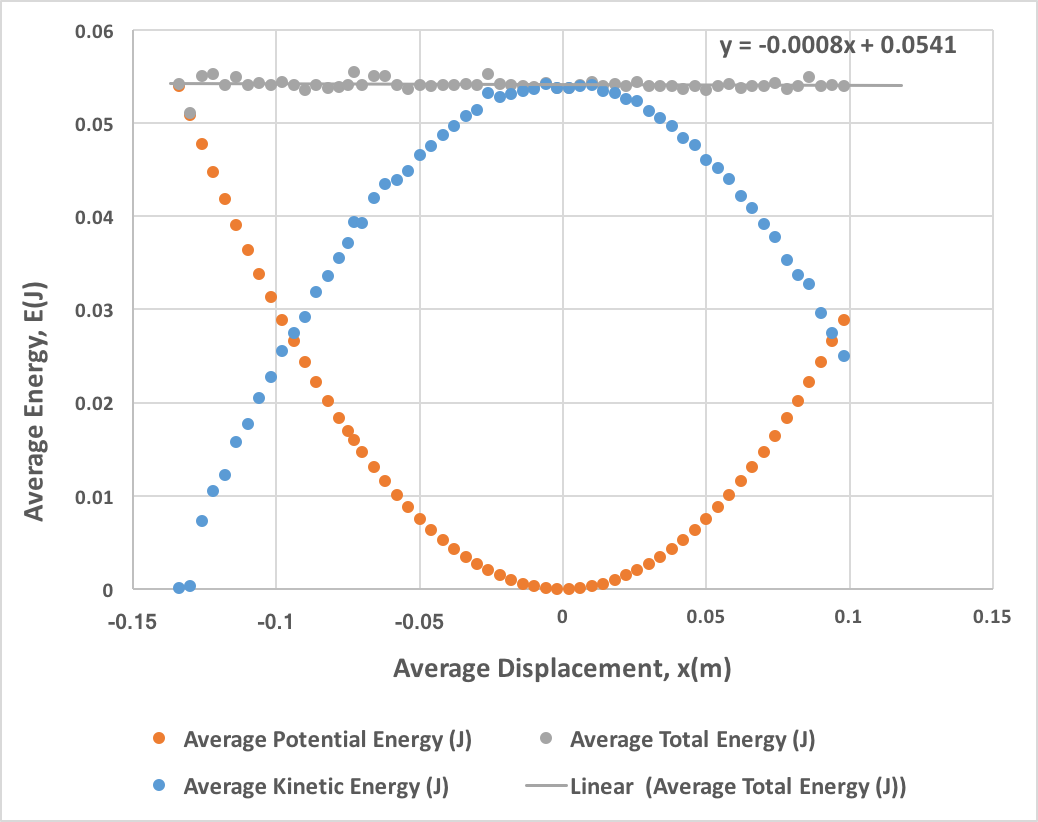
\includegraphics[width=\linewidth]{Energy.png}
    \captionsetup[labelformat=empty]
    \caption{\textbf{Figure 3.2 Kinetic, potential, and total energy of a glider
    attached to springs compared to displacement.}  The best fit line of the
total energy is \(E_{total} = (-0.0008 \pm 0.0003)x + (0.054 \pm 0.002)\), in
units of J.}
\end{figure}

\newpage
\setlength{\parindent}{5ex}
The slope of the best fit line calculated in \textbf{Figure 3.2} represents the
energy lost per meter, in units of J/m.  This is equivalent to the friction
force that opposes the motion of the glider. Friction is equal to the
coefficient of friction times the normal force, or \(F_{friction} = \mu
* N\), where \(N\) is the normal force due to gravity.  The normal force is
equal to the weight of the glider, which has a mass of 0.225 kg.  The normal
force \(N\) of the glider is equal to \((0.225 \pm 0.0005)\) kg * 9.8 m/s = \((2.205
\pm 0.005)\) m/s$^2$.  Having found the normal force, we can find the coefficient
of friction, where \(\mu = \frac{F_{friction}}{N} = 0.0004 \pm 0.0002\).


Because the value of $\mu$ is very small, We can see that we the energy lost 
to friction is extremely small because our glider was on an air track designed 
to minimize the coefficient of friction, making our energy loss almost zero.  

% \section*{Extra Credit}
% \addcontentsline{toc}{section}{Extra Credit}

\section*{Report}
\addcontentsline{toc}{section}{Report}

\begin{center}
\title{
    \Large \textbf{\uppercase{Experimental Proof of Conservation of Energy}}
}

T. Ho\footnote{Henry Samueli School of Engineering and Applied Science,
University of California, Los Angeles}
\end{center}

\subsection*{Abstract}
\addcontentsline{toc}{subsection}{Abstract}
We set out to prove the principle of convervation of energy in a closed system.
To accomplish this, we used a glider with a photocomb on top attached to a 
spring was put on top of an airtrack.  We measured the spring constant by
hanging various masses from the spring and measuring the displacement.
We pulled the glider to the right and released it from rest for one-half 
oscillation; the tips of the photocomb passed through a photogate and allowed 
us to measure the displacement of the glider over time.  After measuring the 
distance between each photogate tooth, we differentiated the displacement with 
respect to time to obtain the velocity at each point in time.   With the spring
constant, glider mass, velocity, and displacement, we plotted potential,
kinetic, and total energy of the system with respect to average displacement.
The graph shows the total energy of the system decreasing only very slightly, 
which we can attribute to any remaining friction in the system.  We proved that 
energy is conserved in a closed system.

\end{document}



%-------------------------------------------------------------------------------
% REFERENCES
%-------------------------------------------------------------------------------
% \newpage
% \section*{References}
% \addcontentsline{toc}{section}{References}

% Anand, U., 2010. The Elusive Free Radicals, \textit{The Clinical Chemist,} [e-journal] Available at:<\url{http://www.clinchem.org/content/56/10/1649.full.pdf}> [Accessed 2 November 2013]
% \newline
% \newline

% Biology Forums, 2012. \textit{Normal glomerulus. Acute glomerulonephritis.} [online] Available at: <\url{http://biology-forums.com/index.php?action=gallery;sa=view;id=9284}> [Accessed 23 October 2013].
% \newline
% \newline

% Budisavljevic, M., Hodge, L., Barber, K., Fulmer, J., Durazo-Arvizu, R., Self, S., Kuhlmann, M., Raymond, J. and Greene, E., 2003. Oxidative stress in the pathogenesis of experimental mesangial proliferative glomerulonephritis, \textit{American Journal of Physiology - Renal Physiology,} 285(6), pp. 1138-1148.
% \newline
% \newline

% Chien, C., Lee, P., Chen, C., Ma, M., Lai, M. and Hsu, S., 2001. De Novo Demonstration and Co-localization of Free-Radical Production and Apoptosis Formation in Rat Kidney Subjected to Ischemia/Reperfusion, \textit{Journal of the American Society of Nephrology,} 12(5), pp. 973-982.
% \newline
% \newline

% Couser, W., 1993. Pathogenesis of glomerulonephritis, \textit{Kidney International Supplements,} 42, pp. 19-26.
% \newline
% \newline

% De Gasparo, M., 2002. Angiotensin II and nitric oxide interaction, \textit{Heart Failure Reviews,} [e-journal] Available at:<\url{http://www.ncbi.nlm.nih.gov/pubmed/12379820}> [Accessed 26 October 2013]
% \newline
% \newline

% Edinburgh Renal Education Pages, 2012. \textit{Glomerulonephritis} [online] Available at: <\url{http://www.edrep.org/pages/textbook/glomerulonephritis.php}> [Accessed 25 October 2013].
% \newline
% \newline

% Forbes, J., Coughlan, M. and Cooper, M., 2008. Oxidative Stress as a Major Culprit in Kidney Disease in Diabetes, \textit{Diabetes,} 57(6), pp. 1446-1454.
% \newline
% \newline

% Geeky Medics, 2010. \textit{Glomerulonephritis} [online] Available at: <\url{http://geekymedics.com/2010/10/27/glomerulonephritis/}> [Accessed 25 October 2013].
% \newline
% \newline

% Gryglewski, R., Palmer, R., Moncada, S., 1986. Superoxide anion is involved in the break­down of endothelium derived relaxing factor, \textit{Nature,} 320, pp. 454-456.
% \newline
% \newline

% Halliwell, B., 2001. Free Radicals and other reactive species in Disease, \textit{Encyclopedia of Life Sciences,} [e-journal] Available at:<\url{http://web.sls.hw.ac.uk/teaching/level4/bcm1_2/reading/oxidative_stress/files/Oxidative_stress.pdf}> [Accessed 19 October 2013]
% \newline
% \newline

% Huang, H., Patel, P. and Salahudeen, A., 2001. Lazaroid compounds prevent early but not late stages of oxidant-induced cell injury: potential explanation for the lack of efficacy of lazaroids in clinical trials, \textit{Pharmacological Research,} 41(1), pp. 55-61.
% \newline
% \newline

% Klinger, J., Abman, S. and Gladwin, M., 2013. Nitric Oxide Deficiency and Endothelial Dysfunction in Pulmonary Arterial Hypertension, \textit{American Journal of Respiratory and Critical Care Medicine,} 188(6), pp. 639-646.
% \newline
% \newline

% Lindemann, I., Boettcher, J., Oertel, K., Pasternack, R., Heine, A. and Klebe, G. 2012. Inhibitors of Transglutaminase 2: A therapeutic option in celiac disease, \textit{To be Published,} [e-journal + PDB structure] Available at:<\url{http://www.ebi.ac.uk/pdbe-srv/view/entry/3s3s/summary}> [Accessed 24 October 2013]
% \newline
% \newline

% Mayo Clinic, 2011. \textit{Glomerulonephritis} [online] Available at: <\url{http://www.mayoclinic.com/health/glomerulonephritis/DS00503/}> [Accessed 20 October 2013].
% \newline
% \newline

% McCord, J., Roy, R. and Schaffer, S., 1985. Free radicals and myocardial ischemia. The role of xanthine oxidase, \textit{Advances in myocardiology,} [e-journal] Available at:<\url{http://www.ncbi.nlm.nih.gov/pubmed/2982206}> [Accessed 24 October 2013]
% \newline
% \newline

% National Health Service, 2012. \textit{Causes of glomerulonephritis} [online] Available at: <\url{http://www.nhs.uk/Conditions/Glomerulonephritis/Pages/Causes.aspx}> [Accessed 20 October 2013].
% \newline
% \newline

% Niaudet, P., 2013. \textit{Overview of the pathogenesis and causes of glomerulonephritis in children.} [online] Available at: <\url{http://www.uptodate.com/contents/overview-of- \ the-pathogenesis-and-causes-of-glomerulonephritis-in-children}> [Accessed 21 October 2013].
% \newline
% \newline

% Ronco, P., 2013. \textit{Mechanisms of glomerular crescent formation.} [online] Available at: <\url{http://www.uptodate.com/contents/mechanisms-of-glomerular-crescent-formation}> [Accessed 21 October 2013].
% \newline
% \newline

% Rutchik, J., 2013. \textit{Toxic Neuropathy Clinical Presentation.} [online] Available at: <\url{http://emedicine.medscape.com/article/1175276-clinical#a0216}> [Accessed 26 October 2013].
% \newline
% \newline

% R\&D Systems, 2013. \textit{Technical Information. Ischemia/Reperfusion Injury.} [online] Available at: <\url{http://www.rndsystems.com/cb_detail_objectname_SP96_Ischemia.aspx}> [Accessed 28 October 2013].
% \newline
% \newline

% Salahudeen, A., 1999. Free Radicals in Kidney Disease and Transplantation, \textit{Saudi Journal of Kidney Diseases and Transplantation,} 10(2), pp. 137-143.
% \newline
% \newline

% Sarma, A., Mallick, A. and Ghosh, A., 2010. Free Radicals and Their Role in Different Clinical Conditions: An Overview, \textit{International Journal of Pharma Sciences and Research,} 1(3), pp. 182-192.
% \newline
% \newline

% Shah, S., Baliga, R., Rajapurkar, M. and Fonseca, V., 2007. Oxidants in Chronic Kidney Disease, \textit{Journal of the American Society of Nephrology,} 18(1), pp. 16-28.
% \newline
% \newline

% The University of Utah, Unknown. \textit{Glomerulonephritis} [online] Available at: <\url{http://library.med.utah.edu/WebPath/RENAHTML/RENALIDX.html#8}> [Accessed 25 October 2013].
% \newline
% \newline

% Wang, C. and Salahudeen, A., 1994. Cyclosporine nephrotoxicity: attenuation by an antioxidant -inhibitor of lipid peroxidation in-vitro and in-vivo, \textit{Transplantation,} 58, pp. 940-946.
% \newline
% \newline

% Wang, C. and Salahudeen, A., 1995. Lipid peroxidation accompanies cyclosporine nephrotoxicity: effects of vitamin E, \textit{Kidney International,} 47, pp. 927-934.
% \newline
% \newline

% Weiss, S., 1989. Tissue Destruction by Neutrophils, \textit{New England Journal of Medicine,} 320, pp. 365-376.
% \newline
% \newline



%-------------------------------------------------------------------------------
% SNIPPETS
%-------------------------------------------------------------------------------

%\begin{figure}[!ht]
%    \centering
%    \includegraphics[width=0.8\textwidth]{file_name}
%    \caption{}
%    \centering
%    \label{label:file_name}
%\end{figure}

%\begin{figure}[!ht]
%    \centering
%    \includegraphics[width=0.8\textwidth]{graph}
%    \caption{Blood pressure ranges and associated level of hypertension (American Heart Association, 2013).}
%    \centering
%    \label{label:graph}
%\end{figure}

%\begin{wrapfigure}{r}{0.30\textwidth}
%    \vspace{-40pt}
%    \begin{center}
%        \includegraphics[width=0.29\textwidth]{file_name}
%    \end{center}
%    \vspace{-20pt}
%    \caption{}
%    \label{label:file_name}
%\end{wrapfigure}

%\begin{wrapfigure}{r}{0.45\textwidth}
%    \begin{center}
%        \includegraphics[width=0.29\textwidth]{manometer}
%    \end{center}
%    \caption{Aneroid sphygmomanometer with stethoscope (Medicalexpo, 2012).}
%    \label{label:manometer}
%\end{wrapfigure}

%\begin{table}[!ht]\footnotesize
%    \centering
%    \begin{tabular}{cccccc}
%    \toprule
%    \multicolumn{2}{c} {Pearson's correlation test} & \multicolumn{4}{c} {Independent t-test} \\
%    \midrule    
%    \multicolumn{2}{c} {Gender} & \multicolumn{2}{c} {Activity level} & \multicolumn{2}{c} {Gender} \\
%    \midrule
%    Males & Females & 1st level & 6th level & Males & Females \\
%    \midrule
%    \multicolumn{2}{c} {BMI vs. SP} & \multicolumn{2}{c} {Systolic pressure} & \multicolumn{2}{c} {Systolic Pressure} \\
%    \multicolumn{2}{c} {BMI vs. DP} & \multicolumn{2}{c} {Diastolic pressure} & \multicolumn{2}{c} {Diastolic pressure} \\
%    \multicolumn{2}{c} {BMI vs. MAP} & \multicolumn{2}{c} {MAP} & \multicolumn{2}{c} {MAP} \\
%    \multicolumn{2}{c} {W:H ratio vs. SP} & \multicolumn{2}{c} {BMI} & \multicolumn{2}{c} {BMI} \\
%    \multicolumn{2}{c} {W:H ratio vs. DP} & \multicolumn{2}{c} {W:H ratio} & \multicolumn{2}{c} {W:H ratio} \\
%    \multicolumn{2}{c} {W:H ratio vs. MAP} & \multicolumn{2}{c} {\% Body fat} & \multicolumn{2}{c} {\% Body fat} \\
%    \multicolumn{2}{c} {} & \multicolumn{2}{c} {Height} & \multicolumn{2}{c} {Height} \\
%    \multicolumn{2}{c} {} & \multicolumn{2}{c} {Weight} & \multicolumn{2}{c} {Weight} \\
%    \multicolumn{2}{c} {} & \multicolumn{2}{c} {Heart rate} & \multicolumn{2}{c} {Heart rate} \\
%    \bottomrule
%    \end{tabular}
%    \caption{Parameters that were analysed and related statistical test performed for current study. BMI - body mass index; SP - systolic pressure; DP - diastolic pressure; MAP - mean arterial pressure; W:H ratio - waist to hip ratio.}
%    \label{label:tests}
%\end{table}
